\section{Finite Pulse Definition and Echo Cancellation}
\label{sec:pulse-definition}

We define the finite generalized Lorentzian envelope by
\begin{equation}
    f_{n,c,L}(t)
    =
    \begin{cases}
    \left[1+(t/\tau)^2\right]^{-n}, & |t|\le L/2,\\
    0, & |t|>L/2,
    \end{cases}
    \label{eq:finite-generalized-lorentzian}
\end{equation}
where $L$ is the total pulse duration, $n$ is the shape exponent, and the
relative endpoint amplitude is $c=f_{n,c,L}(L/2)$.  These parameters imply
\begin{equation}
    \tau
    =
    \frac{L/2}{\sqrt{c^{-1/n}-1}}.
    \label{eq:tau-from-cutoff}
\end{equation}
The root-Lorentzian pulse used here corresponds to $n=1/2$.  Its echo version
has a phase inversion at the center,
\begin{equation}
    \Omega_{\mathrm{E}}(t)
    = \Omega_0 f_{n,c,L}(t)s(t),
    \qquad
    s(t)=
    \begin{cases}
    +1,&t<0,\\
    -1,&t\ge0.
    \end{cases}
    \label{eq:echo-pulse-definition}
\end{equation}
The value assigned at the single point $t=0$ has no effect in the continuum
limit.  In a sampled waveform, the two halves are constructed with equal
duration and opposite phase.

Two cutoff scans must be distinguished.  A pure truncation scan keeps
$\tau$, $n$, and $\Omega_0$ fixed while changing $L$.  A fixed-duration
hardware scan instead keeps $L$ fixed and changes the endpoint ratio $c$; in
the parametrization of Eq.~\eqref{eq:tau-from-cutoff}, this also changes
$\tau$.  Results from these two scans need not coincide.

In the rotating-wave approximation, the unitary two-level Hamiltonian is
\begin{equation}
    \frac{H(t)}{\hbar}
    =\frac{1}{2}\left[\Delta\sigma_z
    +\Omega_{\mathrm{E}}(t)\sigma_x\right].
    \label{eq:echo-two-level-hamiltonian}
\end{equation}
At exact resonance, Hamiltonians at different times are proportional to the
same operator and therefore commute.  The propagator is
\begin{equation}
    U(\Delta=0)
    =\exp\!\left[-\frac{i\sigma_x}{2}
      \int_{-L/2}^{L/2}\Omega_{\mathrm{E}}(t)\,dt\right]
    =\mathbb{I},
    \label{eq:resonant-echo-cancellation}
\end{equation}
because the signed areas of the two symmetric halves cancel.  For
$\Delta\ne0$, the $\sigma_z$ and $\sigma_x$ terms do not commute, so the
cancellation is incomplete and a narrow detuning-dependent response remains.
Equation~\eqref{eq:resonant-echo-cancellation} is exact only for a symmetric,
unitary two-level pulse.  Relaxation, dephasing, phase or amplitude imbalance,
and finite waveform bandwidth prevent exact cancellation in the experiment.

\subsection{Numerical illustration of the echo mechanism}

Figure~\ref{fig:echo-mechanism-simulation} shows the numerical qubit-state
evolution for the root-Lorentzian pulse and its echo variant.  At resonance,
the drive produces coherent evolution during the first half of the echo pulse.
The $\pi$ phase inversion reverses this evolution during the second half, so
the ideal symmetric sequence returns the qubit to its initial state.  In the
open-system simulation the return is incomplete because relaxation and
dephasing act throughout the pulse, consistent with the limitations of
Eq.~\eqref{eq:resonant-echo-cancellation}.

For nonzero detuning, the $\Delta\sigma_z$ term does not reverse at the pulse
midpoint and does not commute with the driven evolution.  The two pulse halves
therefore fail to cancel, leaving a detuning-dependent final population.  The
contrast between the resonant return and the off-resonant response produces
the central depletion feature used to identify the qubit transition.

\begin{figure}[!ht]
    \centering
    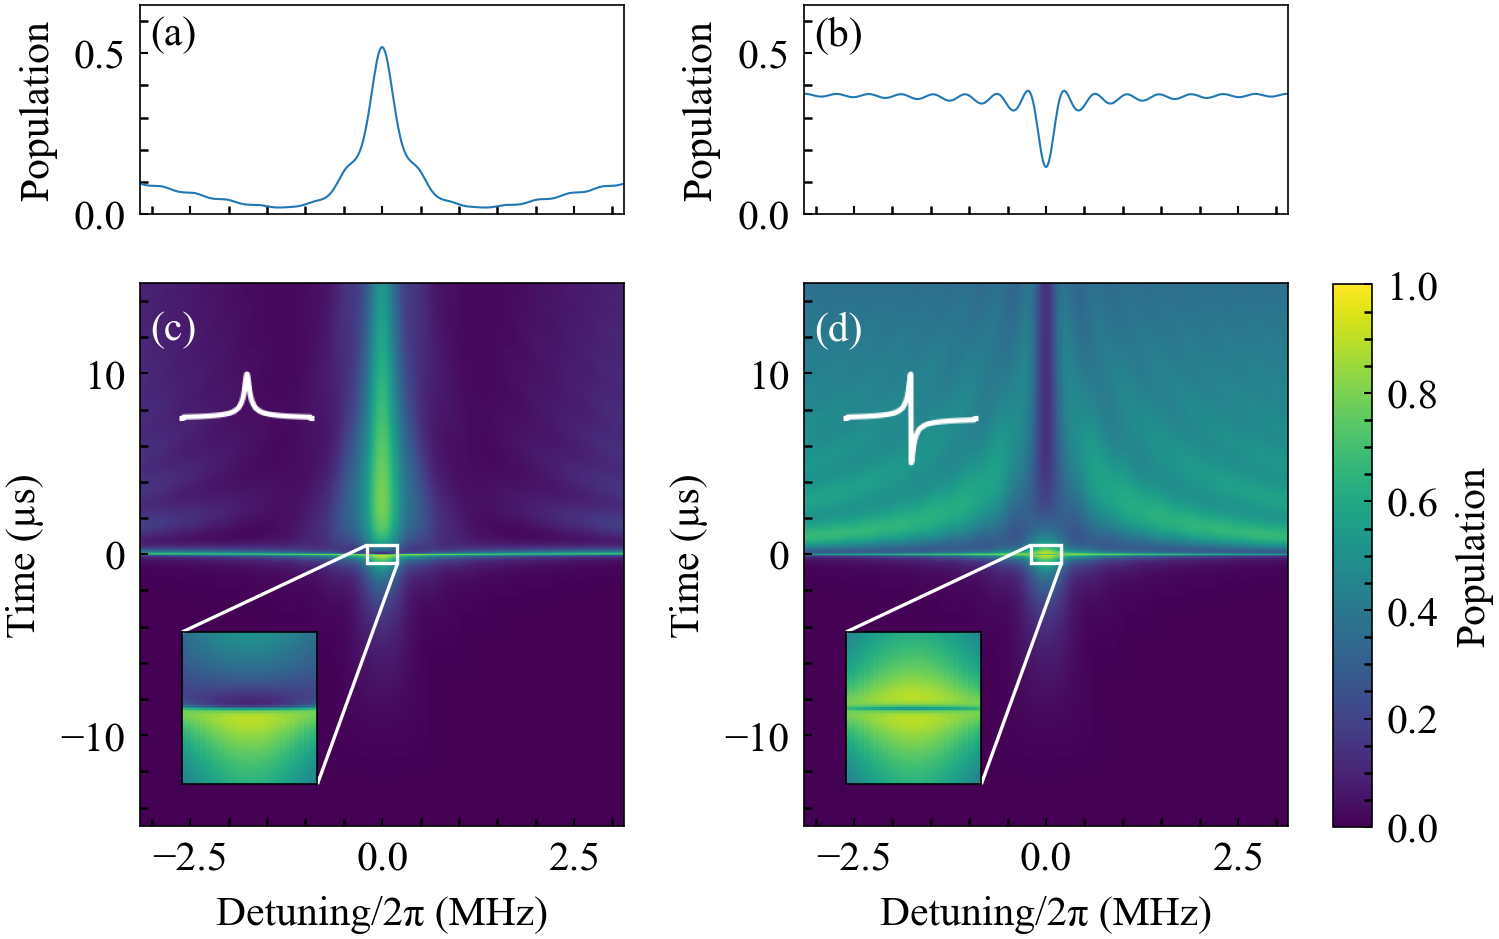
\includegraphics[width=\linewidth]{figures/2d_spectroscopy_simulation.png}
    \caption{Numerical illustration of the echo-cancellation mechanism.
    (a) Final excited-state population versus detuning $\Delta/2\pi$ for a
    root-Lorentzian pulse.  (b) Corresponding response for the
    echo-root-Lorentzian pulse $L^{(1/2)}_{\mathrm{echo}}$.
    (c,d) Full excited-state evolution versus time and detuning for the two
    protocols.  The pulse duration is $30~\mu\mathrm{s}$ and the relative
    endpoint amplitude is $5\times10^{-4}$.  The ordinary root-Lorentzian
    pulse produces a resonant peak, whereas the phase inversion in the echo
    pulse reverses the resonant evolution and produces a central dip.  At
    nonzero detuning the two halves do not cancel, leaving the off-resonant
    population that forms the spectroscopic response.  These archived arrays
    use the historical coherence parameters documented in
    Sec.~\ref{sec:numerical-model}, rather than the later measurement-linked
    values.}
    \label{fig:echo-mechanism-simulation}
\end{figure}
\FloatBarrier
